\documentclass[10pt,aspectratio=169]{beamer}

%% Theme
\usetheme{Madrid}
\usecolortheme{seahorse}
\setbeamertemplate{navigation symbols}{}
\setbeamertemplate{headline}{}

%% Packages
\usepackage{amsmath, amssymb, amsthm, mathtools}
\usepackage{graphicx}
\usepackage{booktabs}
\usepackage{xcolor}
\usepackage{algorithm}
\usepackage{algpseudocode}

%% Theorem environments (use beamer's, not the article ones)
\setbeamertemplate{theorems}[numbered]

%% Operators
\newcommand{\Div}{\operatorname{div}}
\newcommand{\R}{\mathbb{R}}
\newcommand{\E}{\mathbb{E}}
\newcommand{\W}{\mathcal{W}}
\newcommand{\norm}[1]{\left\lVert #1 \right\rVert}
\newcommand{\eps}{\varepsilon}

%% Title page
\title[Extended-MFGAN]{Generative Adversarial Networks for Mean Field Games\\
                       with Weakly Non-Separable Hamiltonians}
\author[Ismatov \& Gomes]{Hikmatullo Ismatov \and Diogo Gomes}
\institute[KAUST]{King Abdullah University of Science and Technology (KAUST)}
\date{\today}

%% =================================================================
\begin{document}

\begin{frame}
  \titlepage
\end{frame}

%% =================================================================
\section{Introduction}

\begin{frame}{What is a Mean Field Game?}
A large population of rational agents, each minimising
\[
  J(\alpha) = \E\Bigl[\int_0^T L(x_t, \alpha_t, \rho_t)\,dt + g(x_T,\rho_T)\Bigr]
\]
against the population distribution $\rho_t$.

\medskip

At Nash equilibrium, $(\varphi, \rho)$ satisfy the coupled system
\begin{align*}
  -\partial_t\varphi - \nu\Delta\varphi + H(x,\rho,\nabla\varphi) &= 0 \quad\text{(HJB)} \\
  \partial_t\rho - \nu\Delta\rho - \Div(\rho\,\nabla_p H) &= 0 \quad\text{(FP)}
\end{align*}

\medskip

\textbf{Applications:}
autonomous traffic, financial markets, energy grids, multi-agent RL.

\medskip

\textbf{Computational challenge:}
solving these in high dimensions is hard.
\end{frame}

\begin{frame}{Two families of deep-learning solvers}
\begin{columns}[t]
\begin{column}{0.49\textwidth}
\textbf{GAN-based} (APAC-Net, MFGAN)
\begin{itemize}
  \item Learns $\rho$ \emph{distributionally} via a generator
  \item Wasserstein convergence
  \item BUT requires \textbf{separable} $H$
\end{itemize}

\medskip
\[
  H(x,\rho,p) = H_0(x,p) - f_0(x,\rho)
\]
\emph{Decoupled}
\end{column}
\begin{column}{0.49\textwidth}
\textbf{Physics-informed} (MFDGM)
\begin{itemize}
  \item Minimises PDE residuals
  \item Handles any $H$, separable or not
  \item BUT $L^p$ pointwise only, no rate
\end{itemize}

\medskip
\[
  H(x,\rho,p) = ?
\]
\emph{General; e.g.\ traffic flow}
\end{column}
\end{columns}

\medskip\hrule\medskip

\textbf{The dichotomy:} powerful theory \emph{or} general applicability, never both.

\medskip

\textbf{Question:} can we keep distributional learning + Wasserstein guarantees
\emph{and} extend to non-separable $H$?
\end{frame}

\begin{frame}{Canonical hard example: MFG-LWR traffic flow}
\[
  H(x,\rho,p) = \tfrac{1}{2}\norm{p}^2 - (1-\rho)\,p
\]

The term $(1-\rho)p$ \textbf{couples} density and momentum. \\
The Hopf-Lax formula breaks. \\
APAC-Net cannot be applied. \\
MFDGM works but with no convergence rate.

\medskip

\textbf{We will show:} this Hamiltonian, and a whole class around it,
admits a \emph{provably convergent GAN-based solver} with explicit rate.
\end{frame}

%% =================================================================
\section{Key idea}

\begin{frame}{The key insight}
\begin{block}{Observation}
If $\rho$ is held fixed, any non-separable Hamiltonian becomes separable.
\end{block}

Decompose
\[
  H(x,\rho,p) = \underbrace{H_0(x,p) - f_0(x,\rho)}_{\text{separable base}}
              + \eps \underbrace{R(x,\rho,p)}_{\text{coupling residual}}
\]

\textbf{Effective Hamiltonian} at iteration $k$:
\[
  H^k(x,p) := H_0(x,p) + \eps\, R(x, \rho^k, p)
  \qquad \text{(separable in $(x,p)$!)}
\]

\medskip

A GAN solver can be applied to each $H^k$.
\end{frame}

\begin{frame}{Weakly non-separable Hamiltonians}
\begin{definition}[Weakly non-separable Hamiltonian]
$H = H_0(x,p) - f_0(x,\rho) + \eps\, R(x,\rho,p)$ where:
\begin{itemize}
  \item $H_0$ strongly convex in $p$ (constant $c_0 > 0$)
  \item $f_0$ Lasry-Lions monotone with constant $\lambda > 0$
  \item $R$ Lipschitz in $\rho$ (constant $L_R$) and in $p$ (constant $L_{R,p}$)
\end{itemize}
\end{definition}

\bigskip

\begin{block}{GAN-tractable regime}
\[
  \boxed{\;\eps\, L_R \;<\; \lambda\;}
\]
(Plus a companion condition $\eps L_{R,p}\rho_{\max} < c_0\rho_{\min}$
when $R$ depends on $p$.)
\end{block}
\end{frame}

%% =================================================================
\section{Algorithm}

\begin{frame}{Extended-MFGAN}
\begin{algorithmic}[1]
\State Initialise $\rho^0 \leftarrow \rho_0$
\For{$k = 0, 1, \ldots, K-1$}
  \State $H^k(x,p) \leftarrow H_0(x,p) + \eps\, R(x,\rho^k(x,t),p)$
  \State \emph{Run inner GAN solver on the separable MFG with $H^k$:}
  \[
    (\rho^{k+1}, \varphi^{k+1}) \leftarrow \textsc{APAC-Net}(H^k, f_0, g, \rho_0)
  \]
\EndFor
\State \Return $(\rho^K, \varphi^K)$
\end{algorithmic}

\medskip

\textbf{Cost:}  $K \times $ (one APAC-Net run).
\textbf{Number of outer iterations:}
$K = \lceil \log(1/\delta)/\log(1/\kappa) \rceil$.

\medskip

\textbf{When $\eps = 0$:} $H^k = H_0$, one outer step suffices.
\textbf{Reduces exactly to APAC-Net.}
\end{frame}

%% =================================================================
\section{Main result}

\begin{frame}{The contraction theorem}
\begin{theorem}[Wasserstein-2 contraction]
Under the GAN-tractable condition $\eps L_R < \lambda$:
\[
  \norm{\rho^{k+1} - \rho^*}_{L^2}
  \;\leq\; \kappa\,\norm{\rho^k - \rho^*}_{L^2},
  \qquad
  \boxed{\;\kappa = \frac{\eps L_R}{\lambda}\;}
\]
Consequently $\rho^k \to \rho^*$ in $\W_2$ at the geometric rate $\kappa^k$.
\end{theorem}

\bigskip

\textbf{First} explicit convergence rate for any deep-learning MFG solver
in the non-separable setting.
\end{frame}

\begin{frame}{Proof idea: Lasry-Lions duality}
Compute
\[
  \frac{d}{dt}\int_\Omega \delta\varphi \cdot \delta\rho\,dx,
  \qquad
  \delta\varphi := \varphi_1 - \varphi_2,\;
  \delta\rho := \rho_1 - \rho_2
\]

Six steps:
\begin{enumerate}
  \item Substitute HJB and FP equations
  \item Diffusion terms cancel
  \item Integration by parts on the current
  \item Integrate over $[0,T]$; boundary terms vanish
  \item Decompose $A_0 + C_0$ (convexity) $+ \eps(A_R+C_R)$ (coupling)
  \item Combine with monotonicity of $f_0$
\end{enumerate}

\medskip

\textbf{Result:}
$\lambda\norm{\delta\rho}^2_{L^2} \leq \eps L_R\,\norm{\delta\bar\rho}_{L^2}\norm{\delta\rho}_{L^2}$.

\medskip

Then Banach Fixed-Point Theorem gives the contraction.
\end{frame}

\begin{frame}{Sharpness: rate is tight}
\begin{block}{Proposition (bilinear exactness)}
For $R = \rho\cdot p$ at the uniform equilibrium, the linearised outer map has
operator norm \emph{exactly}
\[
  \kappa = \frac{\eps L_R}{\lambda}.
\]
The Theorem is therefore sharp; no constant can be improved.
\end{block}

\bigskip

\textbf{Proof sketch.}
On the torus, linearise at $\rho^*=1$.
Stationary FP forces $\Delta(\delta\varphi) = 0 \Rightarrow \nabla\delta\varphi = 0$.
Linearised HJB then reduces to
\[
  -\lambda\,\delta\rho + \eps L_R\,\delta\bar\rho = 0,
\]
i.e.\ $\delta\rho = (\eps L_R/\lambda)\,\delta\bar\rho$.
\end{frame}

\begin{frame}{Necessity: explicit divergence}
\begin{block}{Proposition (necessity)}
When $\eps L_R \geq \lambda$, the linearised iteration does not contract:
it stagnates at $\eps L_R = \lambda$ and grows geometrically when
$\eps L_R > \lambda$.
\end{block}

\bigskip

Same example: ergodic MFG on $\mathbb{T}^d$ with $f_0 = \lambda\rho$ and
$R = L_R\rho$.

\bigskip

\textbf{Combined:} the GAN-tractable condition $\eps L_R < \lambda$ is
\emph{necessary and sufficient} for linear convergence (linearised regime).

\bigskip

This sharpness is unusual:
the contraction theorem is not just a bound, it is the actual rate.
\end{frame}

%% =================================================================
\section{Numerical results}

\begin{frame}{Experiment 1: Separable limit ($\eps = 0$)}
\textbf{Predicted:} one outer iteration suffices when $\eps = 0$.

\medskip

\begin{center}
\begin{tabular}{rrll}
\toprule
$\eps$ & $\kappa$ & $\norm{\rho^1-\rho^*}_{L^2}$ & $\norm{\rho^8-\rho^*}_{L^2}$ \\
\midrule
$0.0$ & $0.0$ & $\boldsymbol{0.0}$ & $0.0$ \\
$0.1$ & $0.1$ & $1.4\!\times\!10^{-2}$ & $1.4\!\times\!10^{-9}$ \\
$0.3$ & $0.3$ & $4.2\!\times\!10^{-2}$ & $9.3\!\times\!10^{-6}$ \\
$0.5$ & $0.5$ & $7.1\!\times\!10^{-2}$ & $5.5\!\times\!10^{-4}$ \\
\bottomrule
\end{tabular}
\end{center}

\medskip

At $\eps = 0$, error collapses to machine zero in one step.
For $\eps > 0$, geometric decay matches theory exactly.
\end{frame}

\begin{frame}{Experiment 2: Bilinear MFG-LWR  (two-sided phase transition)}
For $R = \rho p$, the equilibrium momentum is $p^* = 1-\eps$, so
$L_R(p^*) = |1-\eps|$ and
\[
  \kappa = \frac{\eps\,|1-\eps|}{\lambda}.
\]

\medskip

\begin{center}
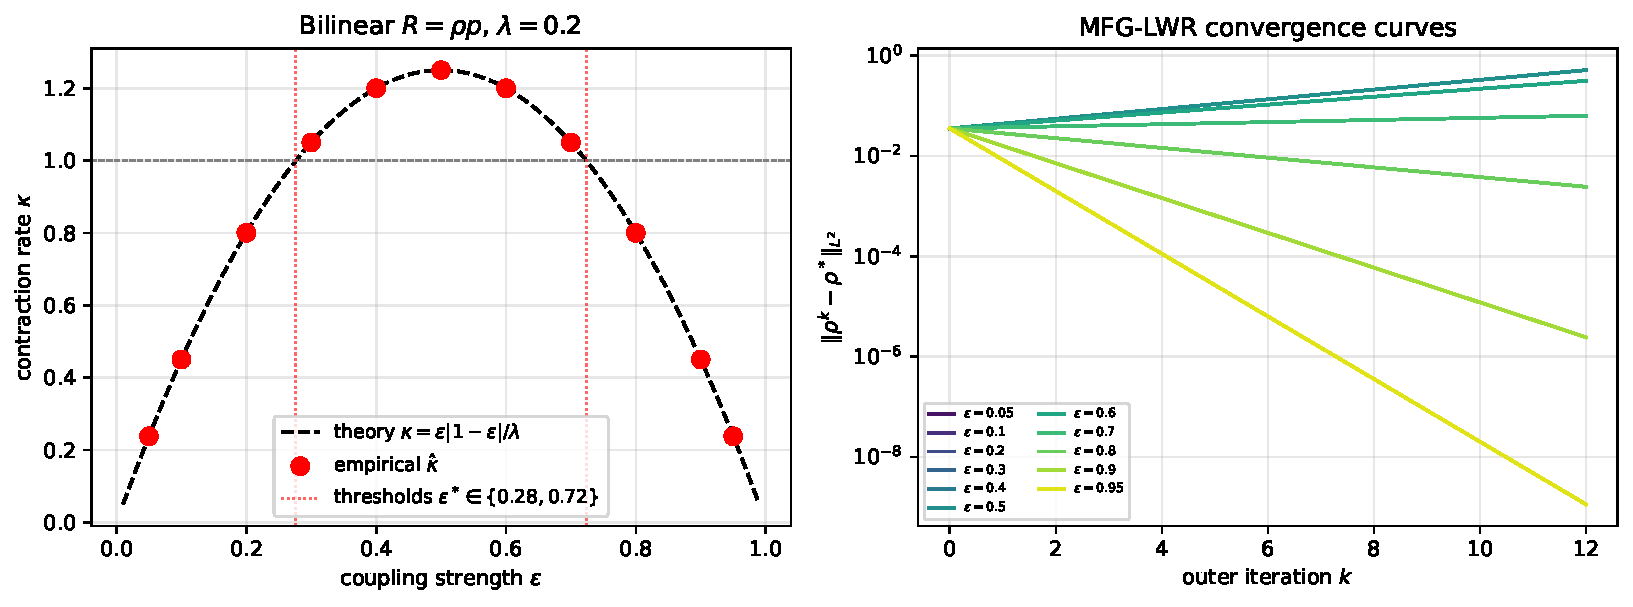
\includegraphics[width=0.92\textwidth]{figures/exp2_traffic.pdf}
\end{center}

Two thresholds at $\eps^*_\pm = \tfrac{1}{2}(1\pm\sqrt{1-4\lambda}) \approx \{0.276, 0.724\}$.
Empirical $\hat\kappa$ matches theoretical $\kappa$ to four digits.
\end{frame}

\begin{frame}{Experiment 3: Single phase transition at $\eps^* = 1$}
Density-only coupling, sweep $\eps \in [0.1, 1.5]$.

\begin{center}
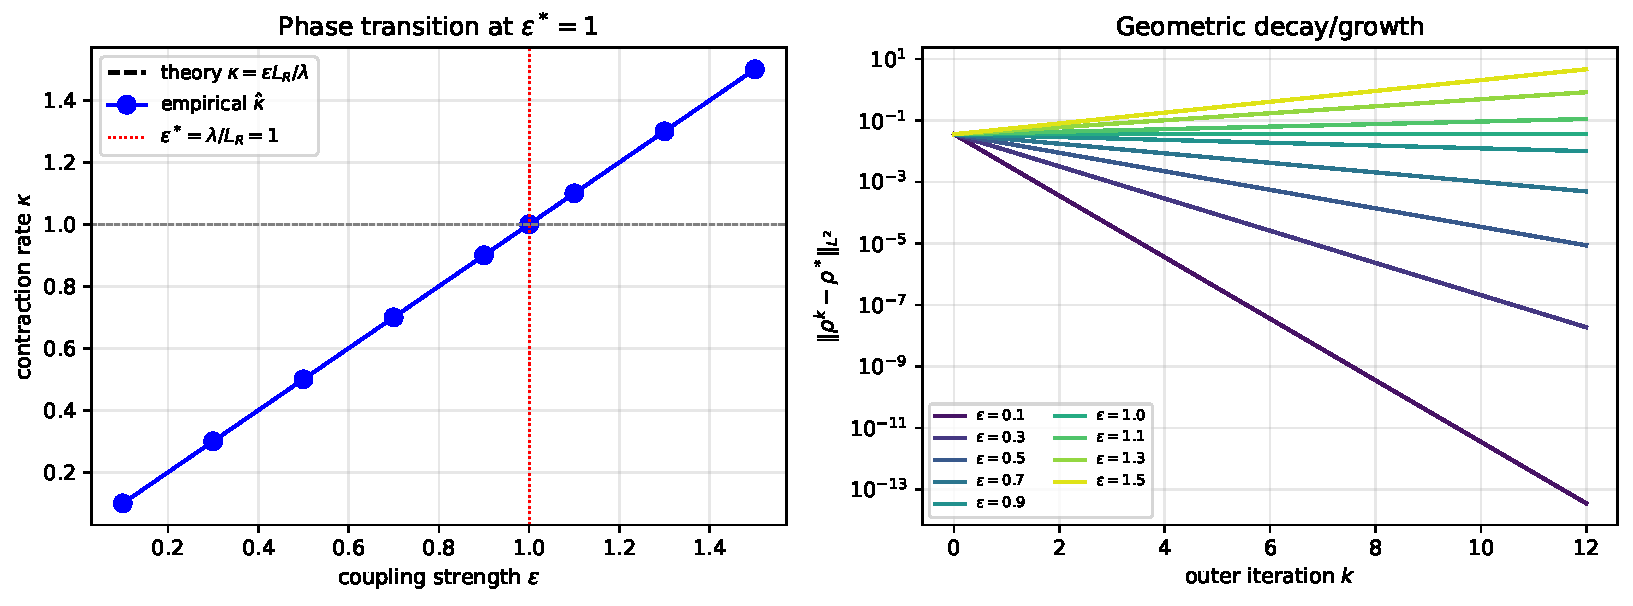
\includegraphics[width=0.92\textwidth]{figures/exp3_phase_transition.pdf}
\end{center}

Empirical $\hat\kappa$ matches theoretical $\kappa = \eps$ to four digits;
sharp transition between geometric decay ($\eps < 1$) and growth ($\eps > 1$).
\end{frame}

%% =================================================================
\section{Wrap-up}

\begin{frame}{Comparison vs prior work}
\begin{center}
\small
\begin{tabular}{lcccc}
\toprule
Method & Non-sep.\ $H$ & $\rho$ representation & Convergence & Rate \\
\midrule
APAC-Net / MFGAN      & No  & Distributional & $\W_1$        & Implicit \\
MFDGM                 & Yes & Pointwise NN   & $L^p$, $p<2$  & None \\
\textbf{Extended-MFGAN} & \textbf{Weak} & \textbf{Distributional} & $\boldsymbol{\W_2}$ & \textbf{Explicit} \\
\bottomrule
\end{tabular}
\end{center}

\medskip

\textbf{Our paper occupies the gap:}
non-separable $H$ + distributional $\rho$ + explicit Wasserstein rate.

\medskip

\textbf{Trade-off:} restricted to weakly non-separable $H$ with
$\eps L_R < \lambda$.
Beyond this threshold, MFDGM is preferred.
\end{frame}

\begin{frame}{Conclusions}
\begin{enumerate}
  \item \textbf{Weakly non-separable Hamiltonians.}
        A formal interpolation between separable and non-separable MFGs.
  \item \textbf{Extended-MFGAN algorithm.}
        Decomposes a non-separable MFG into a sequence of separable ones,
        each solved by APAC-Net.
  \item \textbf{Wasserstein-2 contraction theorem.}
        Explicit rate $\kappa = \eps L_R/\lambda$, the first such for
        non-separable MFGs.
  \item \textbf{Sharpness.}
        The rate is tight (Prop.\ 3.2) and the condition
        $\eps L_R < \lambda$ is necessary (Prop.\ 3.3).
  \item \textbf{Numerical validation.}
        Empirical $\kappa$ matches theory to four digits across three benchmarks.
\end{enumerate}
\end{frame}

\begin{frame}{Future work}
\begin{itemize}
  \item Full neural-network implementation of the inner GAN solver.
  \item Head-to-head benchmark vs MFDGM at the implementation level.
  \item High-dimensional scaling ($d \geq 100$).
  \item Hybrid algorithm: GAN inner-solver $+$ MFDGM fallback when
        $\eps L_R \geq \lambda$.
  \item Extension to mean field control problems.
  \item Application to multi-agent reinforcement learning.
\end{itemize}
\end{frame}

\begin{frame}{Thank you}
\centering
\Large
Generative Adversarial Networks for Mean Field Games\\
with Weakly Non-Separable Hamiltonians

\bigskip

Hikmatullo Ismatov  \quad and \quad  Diogo Gomes \\
King Abdullah University of Science and Technology

\bigskip\bigskip

\normalsize
Code, paper, figures: \\
\texttt{github.com/hikmatulloismatov1999/MFG-GAN-Paper}

\bigskip\bigskip

\textbf{Questions?}
\end{frame}

\end{document}
